%
% green.tex -- Satz von Green
%
% (c) 2021 Prof Dr Andreas Müller, OST Ostschweizer Fachhochschule
%
\bgroup
\definecolor{darkred}{rgb}{0.8,0,0}
\begin{frame}[t]
\setlength{\abovedisplayskip}{5pt}
\setlength{\belowdisplayskip}{5pt}
\frametitle{Satz von Green}
\vspace{-20pt}
\begin{columns}[t,onlytextwidth]
\begin{column}{0.48\textwidth}
\begin{theorem}[Green]
\begin{align*}
\int_G
\biggl(
\frac{\partial g}{\partial x}-\frac{\partial f}{\partial y}
\biggr)
\,
dx\wedge dy
&=
\int_{\partial G} f\,dx + g\,dy
\\
\int_G d\alpha
&=
\int_{\partial G} \alpha
\end{align*}
\end{theorem}
\begin{definition}[äussere Ableitung]
Die {\em äussere Ableitung} einer 1-Form $\alpha = f\,dx+g\,dy$ ist
\[
d\alpha
=
\biggl(
\frac{\partial g}{\partial x}
-
\frac{\partial f}{\partial y}
\biggr)
\,
dx\wedge dy
\]
\end{definition}
\end{column}
\begin{column}{0.48\textwidth}
\begin{center}
\def\pone{
	(1,2) to[out=-90,in=180] (2,1)
}
\def\ptwo{
	(2,1) to[out=0,in=-90] (4.5,3)
}
\def\pthree{
	(4.5,3) to[out=90,in=0] (3.5,4)
}
\def\pfour{
	(3.5,4) to[out=180,in=90] (1,2)
}
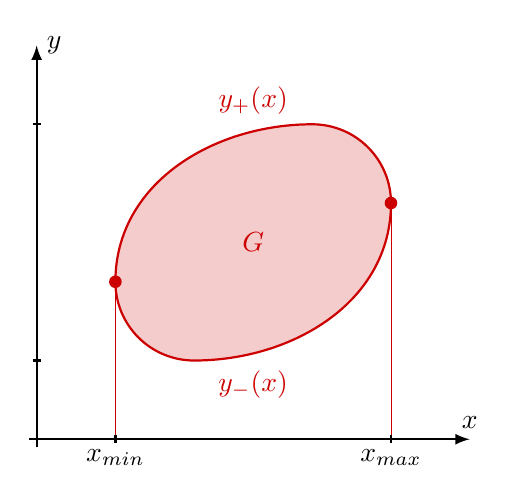
\begin{tikzpicture}[>=latex,thick]
\fill[color=darkred!20] \pone -- \ptwo -- \pthree -- \pfour -- cycle;
\draw[color=darkred] \pone -- \ptwo -- \pthree -- \pfour -- cycle;
\draw[->] (-0.1,0) -- (5.5,0) coordinate[label={$x$}];
\draw[->] (0,-0.1) -- (0,5.0) coordinate[label={right:$y$}];
\fill[color=darkred] (1,2) circle[radius=0.08];
\fill[color=darkred] (4.5,3) circle[radius=0.08];
\draw[color=darkred,line width=0.3] (1,0) -- (1,2);
\draw[color=darkred,line width=0.3] (4.5,0) -- (4.5,3);
\node[color=darkred] at (2.75,2.5) {$G$};
\node[color=darkred] at (2.75,0.7) {$y_-(x)$};
\node[color=darkred] at (2.75,4.3) {$y_+(x)$};
\draw (1,-0.05) -- ++(0,0.1);
\node at (1,0) [below] {$x_{\text{min}}$};
\node at (4.5,0) [below] {$x_{\text{max}}$};
\draw (4.5,-0.05) -- ++(0,0.1);
\draw (-0.05,1) -- ++(0.1,0);
\draw (-0.05,4) -- ++(0.1,0);
\end{tikzpicture}
\end{center}
\end{column}
\end{columns}
\end{frame}
\egroup
